%%%%%%%%%%%%%%%%%%%%%%%%%%%%%%%%%%%%%%%%%%%%%%%%%%%%%%%%%%%%%%%%%%%%%
% LaTeX Template: Project Titlepage Modified (v 0.1) by rcx
%
% Original Source: http://www.howtotex.com
% Date: February 2014
% 
% This is a title page template which be used for articles & reports.
% 
% This is the modified version of the original Latex template from
% aforementioned website.
% 
%%%%%%%%%%%%%%%%%%%%%%%%%%%%%%%%%%%%%%%%%%%%%%%%%%%%%%%%%%%%%%%%%%%%%%

\documentclass[12pt]{report}
\usepackage[a4paper]{geometry}
\usepackage[myheadings]{fullpage}
\usepackage{float} %this is to fix figures at specified location. with [H]
\usepackage{fancyhdr}
\usepackage{lastpage}
\usepackage{graphicx, wrapfig, subcaption, setspace, booktabs}
\usepackage[T1]{fontenc}
\usepackage[font=small, labelfont=bf]{caption}
\usepackage{fourier}
\usepackage[protrusion=true, expansion=true]{microtype}
\usepackage[english]{babel}
\usepackage{sectsty}
\usepackage{url, lipsum}
\usepackage{mathtools}
\usepackage{wrapfig}


\newcommand{\HRule}[1]{\rule{\linewidth}{#1}}
\onehalfspacing
\setcounter{tocdepth}{5}
\setcounter{secnumdepth}{5}

%-------------------------------------------------------------------------------
% HEADER & FOOTER
%-------------------------------------------------------------------------------
\pagestyle{plain}
%\fancyhf{}
%\setlength\headheight{15pt}
%\fancyhead[L]{Ines Wichert}
%\fancyhead[R]{Anglia Ruskin University}
%\fancyfoot[R]{Page \thepage\ of \pageref{LastPage}}
%-------------------------------------------------------------------------------
% TITLE PAGE
%-------------------------------------------------------------------------------
%\usepackage{titlesec}
%\usepackage{sectsty}


\renewcommand\thesection{\arabic{section}.} %define sections numbering
\renewcommand\thesubsection{\thesection\arabic{subsection}} %subsec.num.

%titleformat{\chapter} {\large\scshape}{\thesection}{1em}{}

%titleformat{\section} {\normalfont\scshape}{\thesection}{1em}{}
\begin{document}
\renewcommand\newcounter{section}
\renewcommand\newcounter{subsection}




\title{ \large \textsc{Lab Rotation Report}
		\\ [2.0cm]
		\HRule{0.5pt} \\
		\Large \textbf{\uppercase{pyBREP: A point-cloud based Boundary REPresentation method in python,  applied to finding cell connections}}
		\HRule{2pt} \\ [0.5cm]
		\large Ines Wichert \\ [0.5cm]
		\large April 09, 2018	\\ [0.5 cm]
		\vspace*{5\baselineskip}}

%Talk given January 10, 2017
%Report handed in 
%\date{}

\author{Supervisors: \\ 
	 Dr. Sungho Hong \\
	 Prof. Dr. Erik De Schutter \\
	 BCCN-Intern Supervisor: \\	 
	 Prof. Dr. Richard Kempter\\
		 }
		 
\date{\vspace{-5ex}} %quickfix: remove automatic date. 

\maketitle

\section*{Abstract}
In the large-scale detailed network model used by Sudhakar, Hong et al. in order to investigate in the dynamics of mossy fiber input to the granular layer of the cerebellar cortex, one essential task is to define the morphology of the cells in the model and to find locations at which they are connected. So far, this was done by BREP, a Boundary REPresentation method implemented in Lisp, however this program is not very portable and generally difficult to use, especially without experience in functional programming. Goal of this project was thus to implement pyBREP, a functionally similar python version that is overall easier to apply and work with, yet remains efficient. Following the original BREP, this was achieved by describing cell structures such as the granule cell axon or the Golgi cell dendrites as point clouds, and then using k-d trees to find connections, i.e. points from two different point clouds that are close to each other. In order to speed up the process, a 2D projection method for linear and parallel structures was implemented and the process was parallelized for an IPython Cluster. Connection visualizations and connectivity analysis allow an evaluation of the results and show the comparability with the original BREP. It is hoped that pyBREP will be useful for the current state and further extensions of the cerebellum model, and can also be applied to other network models.

\newpage


\tableofcontents
\newpage

%-------------------------------------------------------------------------------
% Section title formatting
\sectionfont{\scshape}
%-------------------------------------------------------------------------------

%-------------------------------------------------------------------------------
% BODY
%-------------------------------------------------------------------------------




\section{Introduction}

\subsection{A model of the cerebellar granule cell layer}
The cerebellum plays a crucial role in controlling posture and voluntary movement, yet it is also associated to various cognitive functions such as language. Anatomically, it is composed of a cortex and several nuclei. There are three layers of the cortex that can be distinguished: The granule cell layer is the deepest layer, on top of it is the single-cell Purkinje cell layer and the uppermost layer is the molecular layer. In the granule cell layer, the somata of the excitatory granule cells and the inhibitory Golgi cells are located. Granule cell axons ascend through the Purkinje cell layer into the molecular layer (thus, they are called ascending axons) where they branch into two long axon segments that are called the parallel fiber as they run in parallel to each other. Golgi cell dendrites also extend to the molecular layer and get input both from the ascending axons and the parallel fiber. They inhibit the granule cells via their sagittally branching axon, closing a feedback loop between the two cell types. Golgi cells among each other are both connected via their axons that form synapses onto basolateral dendrites of Golgi cells, and gap junctions. Both Golgi and granule cells get input from other brain regions via the so-called mossy fiber. Thus, the granular layer is the first stage of the processing of spatiotemporal input admitted via these fiber. Sudhakar, Hong et al. developed a model of the granule cell layer that investigates in these dynamics and manages to reproduce many of its characteristics see \cite{r:Sudha17}. To this end, the cell types are represented by a model of their morphological structure. Then synapses between them are found, a stimulation is applied and the network behaviour is simulated and recorded using the NEURON simulator \cite{r:NEURON06}.

\subsection{A program to find connected cells}
When setting up the model, the representation of the cell structures and the determination of connections between the cells is a major part. As one of the strenghts of the model is the size of the represented membrane patch, a lot of cells and consequently a lot of connections have to be considered.  Up to now, a program called BREP (Boundary REPresentation language) was used for this task \cite{r:Raikov14}. It is implemented in Scheme, a Lisp dialect, which allows for very fast computation. However, it is not very portable, complicated to set up, and the code might be hard to understand for people who are not used to programming with functional programming languages. Thus, the main goal of the present project was to write a program with a similar functionality as BREP and equal compatibility with the rest of the simulation in python. Further aims were that the code should be efficient, well-documented, and easily understandable. Also, the program should be adaptable and extendable, for example to new cell types, and to also provide extensive possibilities to monitor and investigate its results.



%Sudhakar, Hong et al. developed a rather large-scale detailed network model of the granular layer of the cerebellum. 

%Essentially, the model investigates the interplay of excitatory granule cells and inhibitory Golgi cells, and the influence of inputs such as coming from Mossy fiber. To this end, the cell types are represented by a model of their morphological structure: then synapses between them are found, a certain stimulation is applied and the network behaviour is simulated using the NEURON simulator. Between Golgi and granule cells, there are the following types of connections: \paragraph*{granule cell to Golgi cell:} Both the ascending axon (the part of




 
\section{Implementation of pyBREP}

\subsection{Point cloud representation of the cells}

In order to represent the structure of the different cells, 3-dimensional points with a regular spacing along linear structures are used. In the current case, only Golgi and granule cells have to be represented. If not declared differently, all parameter values in the following section were directly taken from the simulation code that was published in association with \cite{r:Sudha17}.
 

\subsubsection{Golgi cells}
For the Golgi cells, two apical and two basal dendrites are rendered as lines on cones. The base areas of the cones consist of a circle of radius 60 \textmu m for the basolateral, and 100 \textmu m for the apical dendrites, respectively. The height of the cones is 332 \textmu m in z-direction for the apical dendrites, and -6 \textmu m for the basolateral dendrites (with 'height' being the cone's extent in vertical direction, i.e. perpendicular to the layers, towards the molecular layer). The direction of the dendrites in the horizontal plane (i.e. in the plane parallel to the cortex surface) is determined by sampling from a standard distribution around mean values that are the same for each Golgi cell. For the apical dendrites, the mean values are $30^{\circ}$ and $120^{\circ}$ and standard deviation is $50^{\circ}$. For the basolateral dendrites, the distributions are centered on $-20^{\circ}$ and $-240^{\circ}$, with a standard deviation of $1^{\circ}$. Note that, to provide comparability with the original BREP program, a unit vector with a direction of $0^{\circ}$ is defined to be in parallel with the transverse axis, and angles increase in a counterclockwise direction. To take into account the electrophysiological properties of the conductance along the dendrite, each dendrite is segmented into a certain number of segments (5 for apical, 3 for basal), i.e. the segment number is a discretized measure for the distance between a synapse and the soma. Each segment is represented by a certain number of points (5 for apical, 4 for basal dendrites), which are assumed to be equal in their electrophysiological properties. Thus, every point is classified by the ID of the Golgi cell it belongs to, then the number of the dendrite it lies on (1 and 2 for basal, 3 and 4 for apical), and finally the number of the segment that it is part of.
The Golgi cell axons are spread around the Golgi cell soma, with their extension being slightly elongated in sagittal direction. Thus, they are simulated as 20 uniformly distributed random points in a cuboid of extension 90 \textmu m in transverse, 320 \textmu m in sagittal and 150 \textmu m in vertical direction, with the soma, represented by one additional point, in the center of the cuboid.

\begin{figure}[!ht]
	\centering
	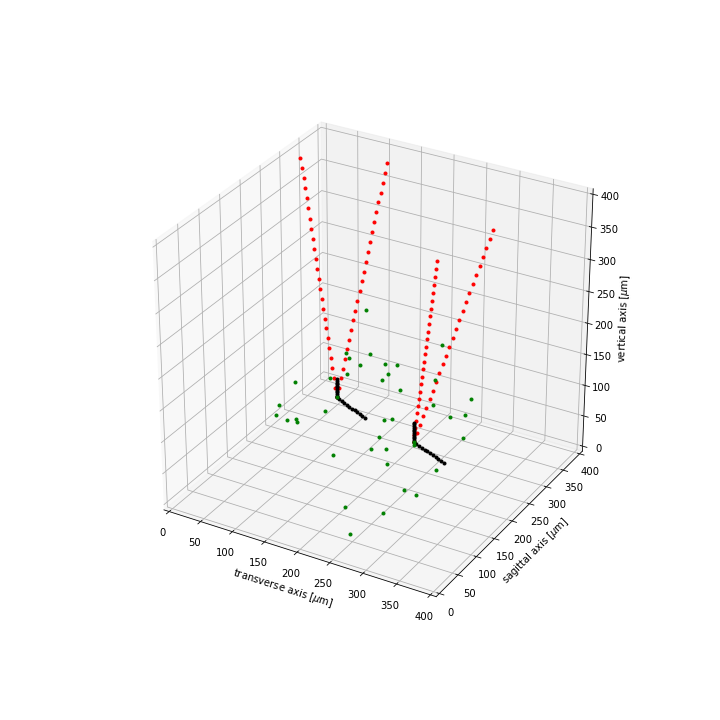
\includegraphics[width=0.8\textwidth]{./figures/two_golgi_cells.png}
	\caption{Model of the dendritic tree of two Golgi cells: Each tree consists of an apical part (red), stretching up until the molecular layer, and a basal part (black), spreading throughout the granule cell layer. Both parts are modelled as points on two straight lines lying on the surface of a cone that has its peak at the Golgi cell soma. The axon is represented by the green points.}
	\centering
	\label{f:two_golgis}
\end{figure}




\subsubsection{Granule cells}
For each granule cell, an ascending axon (AA) stretches along the z-direction from the granular layer to the molecular layer, crossing the Purkinje cell layer. At its end it branches into the parallel fiber (PF), running in transverse direction, with a length of 1000 \textmu m in each direction. In the current simulation, the length of the AA is fixed at 230 \textmu m, although there is an additional option implemented that chooses the lenght of the AA to end at a random height of the molecular layer.

% As recent data ***(who?, personal communication) suggests that the location of the granule cell body is rather independent of the height of its branching point in the molecular layer, an additional option was implemented to randomly choose the length of the AA, as long as it ends in the molecular layer.  

\begin{figure}[!ht]
	\centering
	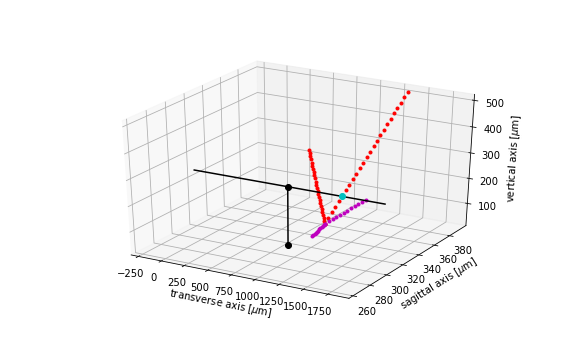
\includegraphics[width=0.8\textwidth]{./figures/pf_gol_con_single.png}
	\caption{Golgi and granule cell together. The Golgi cell is connected to the parallel fiber of the granule cell. Note that the figure axes are distorted in order to fit the whole parallel fiber.}
	\centering
	\label{f:gol_gran_con}
\end{figure}


\subsection{K-d trees allow efficient nearest neighbour searches}

\subsubsection{Concept}
K-d trees \cite{r:Bentley75} are binary search trees that embed points in a k-dimensional space. 
In order to build such a tree on a set of points, an arbitrary starting point is chosen. Then, a hyperplane is defined that is perpendicular to one of the spatial dimensions. It separates all points into a left and a right subtree, depending on which side of the hyperplane they are on. The points in the subtrees are then seperated again, each by a hyperplane that is perpendicular to the previous one. This is repeated, whereby the hyperplanes are perpendicular to an axis that is determined in a circulating way, until there is only one node left in each subtree.

\begin{figure}[!ht]
	\centering
	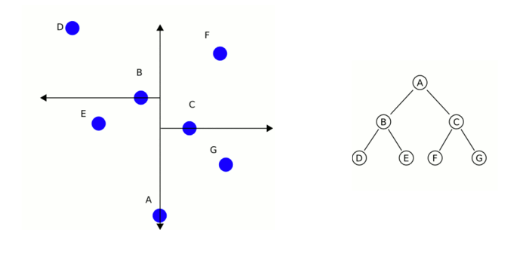
\includegraphics[width=0.8\textwidth]{./figures/kd_tree2.png}
	\caption{Scheme of a small 2D tree. Left: Tree points, Right: Tree. A is the root node, and thus the first separating hyperplane runs through it, splitting the remaining points in two subtrees. B and C are the next levels, their separating hyperplanes are orthogonal to the first. Adapted from \cite{r:kdt}}
	\centering
	\label{f:kdt}
\end{figure}

When searching for a nearest neighbor of a query point, one first moves down the tree. For each node, a check is performed which side of the hyperplane that goes through the node contains points that are closer to the query point (i.e., the side on which the query point is lying is chosen). This is performed until a leave node is reached. There is always a current best node, and whenever a node is visited that is closer to the query point, this node is saved as the new current best. Then, the algorithm moves up the tree again. This time, for every node it is checked, whether the other side of the hyperplane which goes through the point could contain a point that is closer to the query point as the current best, which is the case if the hyperplane intersects with a hypersphere around the query point with a radius of the current best distance. If there is an intersection, the algorithm moves down the other subtree, again updating the current best if adequate. When it arrives at a leave node point, the algorithm starts walking up the tree again. This iterative process terminates when the algorithm walks back up until the root node. 

In order to find all points within a certain critical radius, a similar search is performed, although this time all points that lie within this radius are stored, and obviously the radius is not changed because of an identified nearer point.


\subsubsection{Application and parallelization}
In pyBREP, connections between two cell populations have to be found. The points representing one population are thus organized in a k-d tree, and the points representing the other population are used as query points. The critical distance, i.e. the distance at which two points from different populations connect, is implemented as the radius around the query point in which tree points are searched. As it is faster to query few points in a big tree than many points in a small tree, the program per default determines the population that is described by more points and stores it in the tree.
To further speed up the process and make effective use of computing power, the search process can be parallelized. This is in this case done on an IPython-Cluster, using the libraries ipyparallel \cite{r:ipp} and cloudpickle \cite{r:cloudpickle}. Each cluster unit, or worker, receives a copy of the k-d tree containing the bigger point cloud. The other point cloud is then distributed so that every worker receives a roughly equal amount of points. The workers then perform the search for the points they are responsible for and save their results independently.

\subsection{2D projections}
Due to their elongated structure, granule cells are represented by more than 200 points, which leads to a high computational burden.
However, both the ascending axon and the parallel fiber run in parallel to an axis. In the used convention, it is the vertical (z) axis for the AA, and the transverse (y) axis for the PF. Thus, a simple projection can be performed by representing each structure as its intersection point with the plane perpendicular to it (fig. \ref{f:proj_2D}). Thus, a 2-dimensional tree can be used to find connections, and as they are now only represented by one point, it is sufficient to only perform one nearest neighbour search per AA or PF. Only one additional comparison in the omitted coordinate axis is necessary to check whether the single projected points lie within the range of the linear structure. This method thus strongly increases both speed and resource efficiency.
Apart from these advantages, this method leads to a homogenate connection density along the linear structure, as the region in which connections are found is cylindrical rather than bead-like.
However, this method can only be applied to linear structures that are parallel with each other, such as granule cells in our case. Consequently, also the 3D method is available in pyBREP, which can be used on more complex structures.

\begin{figure}[H]
	\centering
	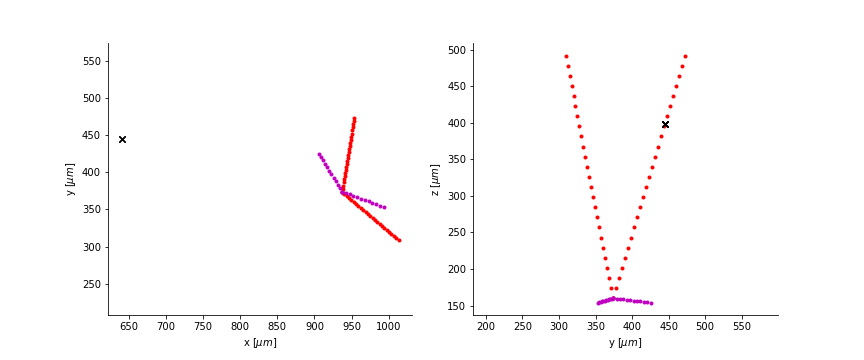
\includegraphics[width=0.8\textwidth]{./figures/projected_2D.png}
	\caption{The same cells as in fig. \ref{f:gol_gran_con} are represented as their projections. Left: the x-y plane projection of the ascending axon of the granule cell (black x) cannot intersect with the Golgi cell dendrites (red dots). Right: The y-z plane projection shows that the parallel fiber of the granule cell (black x) might intersect with the Golgi cell dendrites. Now the x-coordinates of the respective Golgi cell dendrite point must be compared with the extension of the parallel fiber to decide whether a connection is formed.}
	\centering
	\label{f:proj_2D}
\end{figure}
 
%Instead, a projection method was developed that allowed the representation of the ascending axon and the parallel fiber by one single point respectively.
%As for the particular given geometry of the granule cellsthe elongated structure of the granule cells leads to a lot of points and thus to a big computational effort, an alternative of the 

\subsection{Flexibility and extendability through a modular structure}
To keep the program flexible and make it easy to extend, the rendering of the cells is seperated from the connection part. Figure \ref{f:structure} gives an overview over the main structure. Cell populations are represented by classes such as Golgi\textunderscore pop or Granule\textunderscore pop, both inheriting from a basic Cell\textunderscore pop class. They are used to render the point clouds that represent the cell structures. These are then organized as Query\textunderscore point class objects, which assemble their coordinates with optional additional information such as corresponding cell IDs, segment numbers, or distance offsets. Two Query\textunderscore point objects (or, alternatively, regular numpy arrays) are then passed to a connector class, which finds points of the two different point clouds that are close to each other, and registers them as cell connection. Depending on the geometry of the point clouds, the Connect\textunderscore 2D class can be used (using 2D projections, for example to find connections between parallel fiber and Golgi cell dendrites), or the Connect\textunderscore 3D class (e.g. for inhibitory connections between Golgi cells). Both classes can, but do not need to work in parallel.
All three class types - cell populations, point clouds, and connectors - can be extended independently from the other ones. For example a cell type could be added and connected to the already existing cell types using the same connectors. This modular structure makes pyBREP flexible and adaptable to a wide range of detailed (neuronal) networks.
%Query\textunderscore point objects are an output of the population classes, and they are the input for the connector classes. It is also possible to pass numpy arrays as arguments to the Connector objects, but they will then be automatically turned into Query\textunderscore point objects. 
%Thus, for the planned implementation of other cells that connect to the parallel fiber, hopefully only an additional cell population class has to be implemented.
%The Connector classes will connect the data either by using the 2D projection method as in the case of the Connect\textunderscore 2D class, or with the orignal method using 3D Trees as in the case of the Connect\textunderscore 3D class. Both classes can, but don't have to work in parallel. 
Results are saved split up in four file types:
'\textunderscore source' files contain the cell (or point) ID of the source population, '\textunderscore target' the IDs of the target population. The '\textunderscore segments' and '\textunderscore distance' files contain information about the location of the connection with respect to the connected cells, which has to be taken into account electrophysiologically. 


\begin{figure}[!ht]
	\centering
	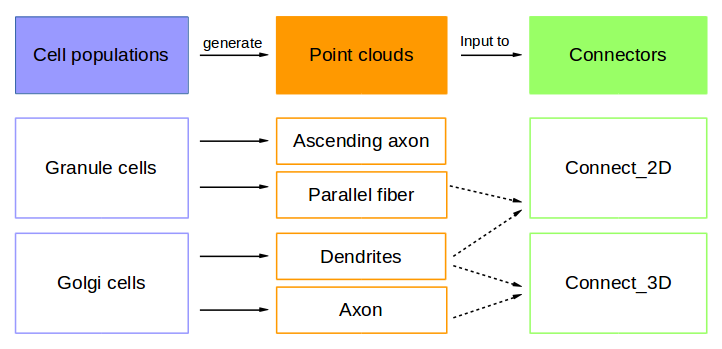
\includegraphics[width=0.8\textwidth]{./figures/pyBREP_structure.png}
	\caption{Overview over the structure of pyBREP. Cell population classes generate point clouds representing morphological structures. Those point clouds are then fed into Connectors that find connections, i.e. points from different point clouds that are close to each other. In each of the three columns, new types can be added and integrated independently from the other columns.}
	\centering
	\label{f:structure}
\end{figure}

%In the case of the Connect_2D class, the '_segments' files contain the dendrite and segment number of the population that remains in its 3-dimensional structure, in the Connect_3D class it is currently the information 
%Thus, the parts of the program that actually find the connections can be applied to coordinate data in a variety of formats. 

\section{Evaluation and Testing}
As a proper functionality of this program is crucial for the overall simulation, a set of methods to control and evaluate its results is necessary. 
A first set of methods targets single cells and checks its connections in oder to make sure that only close-by cells are found. 
A second set of methods analyzes the connectivity, i.e. the number of connections that each cell forms.  %When testing code, often a smaller chunk of cerebral cortex was used, generated by dividing the lengths of the transverse and sagittal axis by 4, and only using the cells within this smaller region.

\subsection{Single cell connections}
In this part, the functionality of the connectors is evaluated by choosing a single cell and displaying all cells that were found to be connected to it. For the Connect\textunderscore 3D class this is done by finding inhibitory Golgi-Golgi interactions, i.e. connections between the Golgi cell axons and dendrites. Figure \ref{f:gogo_conn} shows that only Golgi cells in the proximity of the selected Golgi cell are found, an indicator for the overall correct function of the Connect\textunderscore 3D class.

\begin{figure}[!ht]
	\centering
	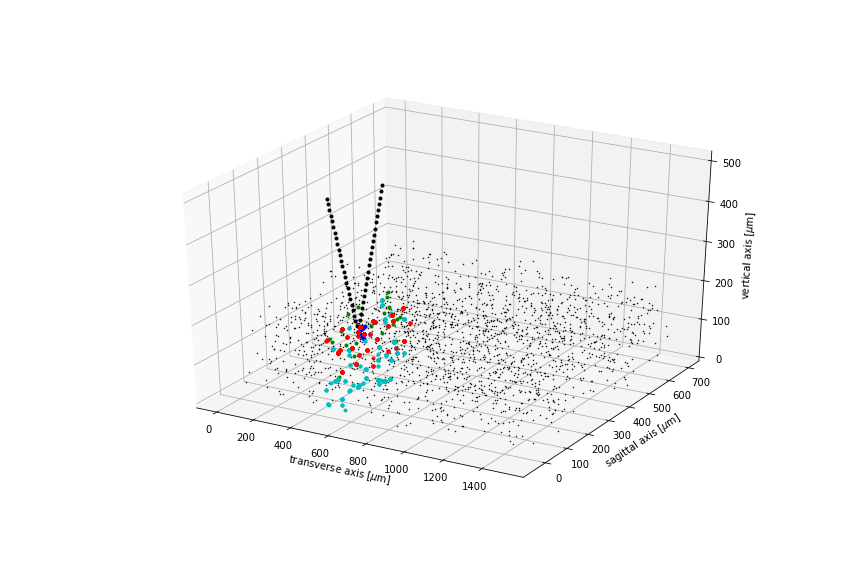
\includegraphics[width=0.8\textwidth]{./figures/gogo_one_cell_conn.png}
	\caption{Inhibitory connections between Golgi cells: Each Golgi cell of the simulation is represented by a small black dot. One Golgi cell is represented in its full morphology (apical dendrites: big black dots, basal dendrites: blue dots, axon: green dots). All the Golgi cells connected to it are represented as red dots (cells that give input), or blue dots (cells that receive input). Note that they are only possible connections, when the simulation is set up, a Boltzmann distribution depending on the cell distance gives the probability that the connection is actually read in.}
	\centering
	\label{f:gogo_conn}
\end{figure}


For the Connect\textunderscore 2D class, connections between Golgi cells and granule cells are investigated. Figure \ref{f:pf_gol_conn} displays this for a smaller membrane patch. The connected granule cells lie within defined regions which reflect their morphology, which is an indicator for the correct function of the class. 


\begin{figure}[h!]
\begin{minipage}[r]{16cm}
\vspace{0pt}
\centering
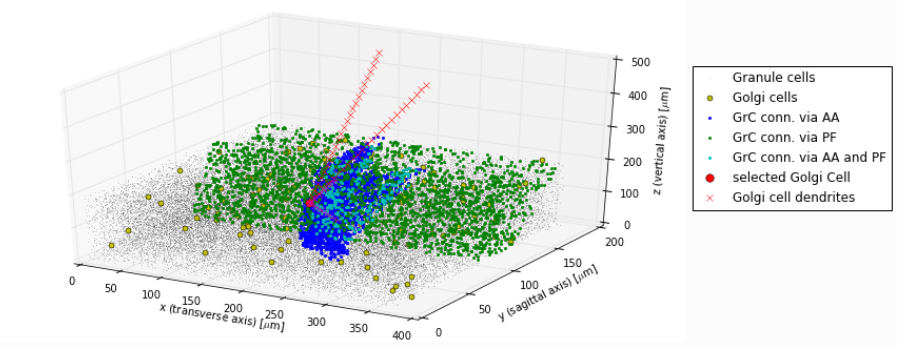
\includegraphics[width = 15cm]{./figures/gol_gran_allconn.png}
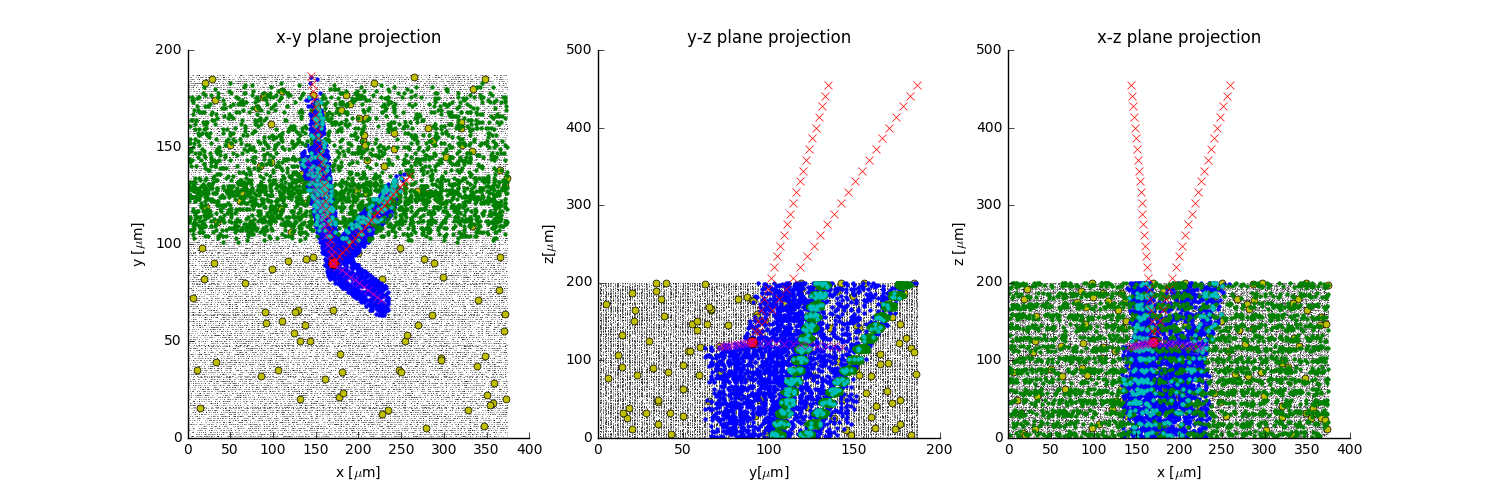
\includegraphics[width = 15cm]{./figures/gol_gran_allconn_proj.png}
\end{minipage}
\hfill
\caption{Granule cells connected to one particular Golgi cell (red). Upper: 3D model, lower: 2D projections. A smaller patch of the membrane is used, all granule cells are depicted as little black dots, all Golgi cells as bigger yellow ones. The granule cells that are connected to the selected Golgi cell are colored green if the connection is via their parallel fiber; blue, if it is via the ascending axon; and cyan if it has both types of connections.}
\label{f:pf_gol_conn}
\end{figure}


Using these methods, issues such as duplicate connections or self-connections were reveiled. As they can also be found in the output of the original BREP, these issues were not given a high priority, however they will be addressed as possible improvement in section \ref{s:todo}.


\subsection{Connectivity analysis}
\label{s:conn_an}

After single cell level methods, connectivity analysis is performed on population level. To this end, the number of connections per cell is counted and then represented in a histogram over the population. As a first step, this histogram was compared to the corresponding histogram of the output of the original BREP program. This lead to the insight that the critical radius, i.e. the distance at which two points are considered linked together had to be adapted to 2.5 $\mu m$ for the ascending axon, and to 3.5 $\mu m$ for the parallel fiber. This decrease in comparison to the original program can be explained by taking into account that with the 2D projection method, the region in which connections are found is cylindrical rather than bead-like. Thus, at the same critical radius, its volume is bigger. Figure \ref{f:pf_gol_hists} shows the pyBREP output with the adapted radius, and the original BREP output. 

\begin{figure}[h!]
\begin{minipage}[r]{16cm}
\vspace{0pt}
\centering
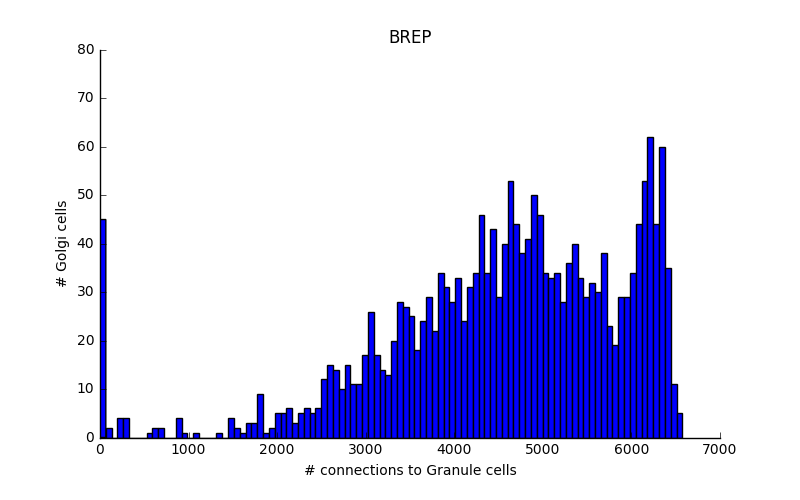
\includegraphics[width = 7.5cm]{./figures/brep_pf_golgi_hist.png}
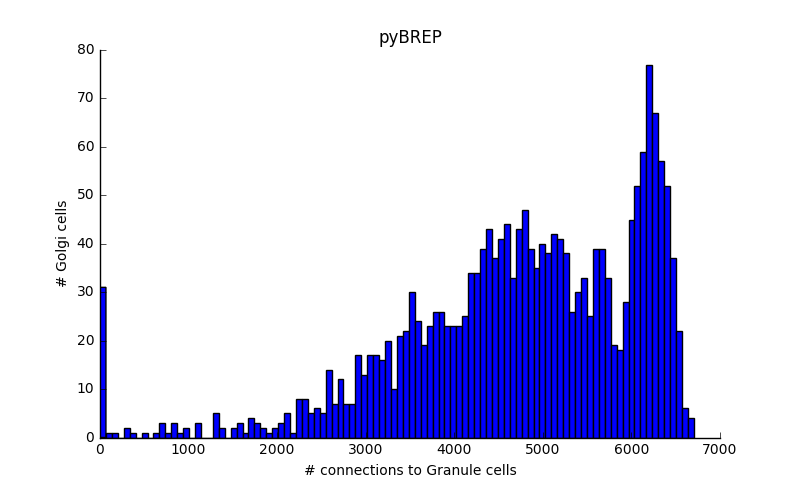
\includegraphics[width = 7.5cm]{./figures/pybrep_pf_golgi_hist.png}
\end{minipage}
\hfill
\caption{Histograms depicting the number of connections that a Golgi cell has with parallel fibers. Left: Original BREP solution. Right: pyBREP solution.}
\label{f:pf_gol_hists}
\end{figure}

Both the original BREP and pyBREP have a second histogram peak that we wanted to understand better. So we went into more detail and visualized all Golgi cells, color-coded by the number of their parallel fiber connections (fig. \ref{f:gol_scatter}). The visible inhomogeneities in the horizontal plane can be explained as for a high number of cells, the dendrites reach out of the simulated patch of membrane and are thus 'cut'. Along the vertical axis, only the apical dendrites of the Golgi cells in the upper half can reach completely through the molecular layer, consequently they have more connections. Taken together, the group of cells that have dendrites that span maximally throughout the upper layer and are not cut on either side are the group of cells that are contained in the second peak of the histogram.  

\begin{figure}[H]
\begin{minipage}[r]{14cm}
\vspace{0pt}
\centering
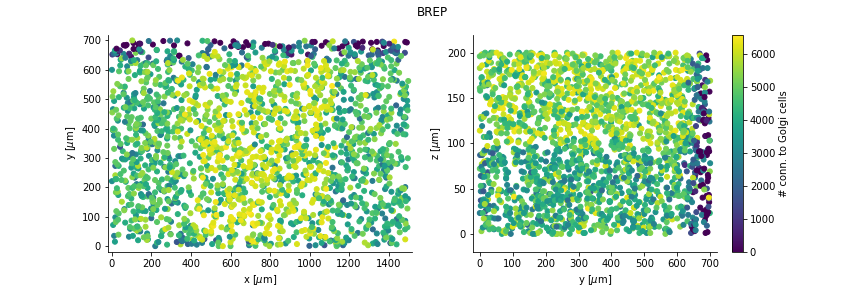
\includegraphics[width = 14cm]{./figures/brep_golgi_scatter.png}
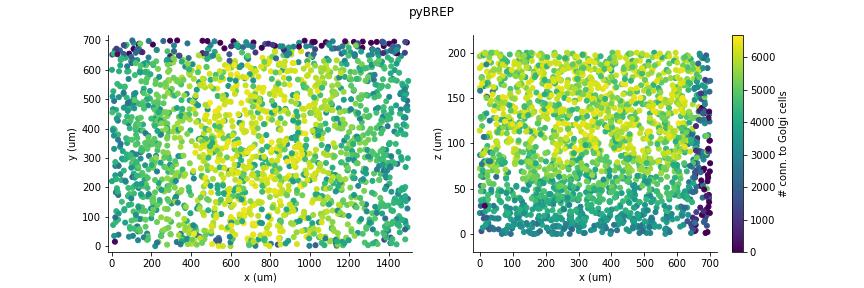
\includegraphics[width = 14cm]{./figures/pybrep_gol_scatter.png}
\end{minipage}
\hfill
\caption{Histograms depicting the number of connections that a Golgi cell has with parallel fibers. Upper: Original BREP solution. Lower: pyBREP solution.}
\label{f:gol_scatter}
\end{figure}

\begin{figure}[H]
\begin{minipage}[r]{14cm}
\vspace{0pt}
\centering
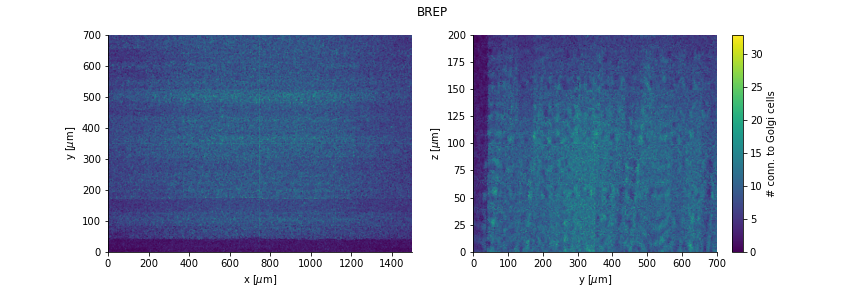
\includegraphics[width = 14 cm]{./figures/brep_pf_scatter.png}
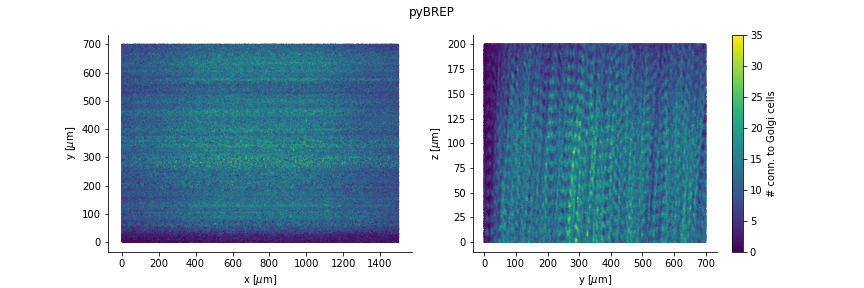
\includegraphics[width = 14 cm]{./figures/pybrep_pf_scatter.png}
\end{minipage}
\hfill
\caption{Histograms depicting the number of connections that a Golgi cell has with parallel fibers. Upper: Original BREP solution. Lower: pyBREP solution.}
\label{f:pf_scatter}
\end{figure}

When checking the other way around, i.e. color-coding granule cells by the number of connections that they form with Golgi cells via their parallel fiber, a different kind of inhomogeneity can be seen ( fig. \ref{f:pf_scatter}). Slightly tilted bead-like stripes of cells with more connections are visible in the y-z plane projection. This is likely due to Golgi cells that are spaced in a way that the connecting regions of their dendrites overlap in some axis. Consequently, granule cells that connect to one of them are likely to also connect to the other ones, and have more connections. The pattern can be seen both in the pyBREP and the original BREP solution, but it is stronger in the pyBREP one. A likely cause for that is that in the original BREP, Granule cell axons were also represented by 3-dimensional dots at a certain spacing, so there is one more axis where they would have to be aligned. That blurries the pattern.  
 
%A likely cause for that was identified: The soma locations of the cells are not chosen entirely randomly, they are calculated by having a regular spacing to which a random component is added. As the spacing between the Golgi cell dendrite points that are able to find connections also has a certain rhythmicity, the patterns in connectivity are likely to be interference patterns of the Golgi cell dendrite spacing and the spacing between the different cell somate. This was checked by writing a new, more random algorithm to generate cell soma points and to rerun the algorithm on that. Indeed, the patterns could no longer be found. However, the second used algorithm was not really based on any morphological knowledge. Thus, an improved algorithm to generate the locations of the cells or another solution to this problem would be a high priority task for further improvement (\ref{s:todo})

The same analysis was performed for ascending axons (not displayed).

%To go more into detail, gain an overview over the spatial distribution of the cells, and especially understand the second peak of the histogram, Golgi cells were represented as circles, with the number of connections color-coded as the circle filling. This was represented both as a 3-dimensional plot as well as as the 3 possible 2D-projections.

%Certain inhomogeinities were expected- for example, Golgi cells with dendrites that reach out of the chunk are expected to have less connections, and for parallel fiber connections, Golgi cells that lie rather low in the slice also  should have less connections as their apical dendrites do not span the whole molecular layer. However, there were also some unwanted regularities: There were two stripes of cells with more connections. After repeated and detailed checking of the code, a very likely cause was identified: The soma locations of the cells are not chosen entirely randomly, they are calculated by having a regular spacing upon which a random component is added. As the spacing between the Golgi cell dendrite points that are able to find connections also has a certain rhythmicity, the patterns in connectivity are likely to be interference patterns of the Golgi cell dendrite spacing and the spacing between the different cell somate. This was checked by writing a new, more random algorithm to generate cell soma points and to rerun the algorithm on that. Indeed, the patterns could no longer be found. However, the second used algorithm was not really based on any morphological knowledge. Thus, an improved algorithm to generate the locations of the cells or another solution to this problem would be a high priority task for further improvement (\ref{s:todo})



\section{Outlook: Further steps for the current program}
\label{s:todo}
The pyBREP implementation existing to date is tailored to the simulation in its current form. A first important part of evaluation would thus be to let the full simulation run using it and compare the results to results that have been obtained using the original BREP. However, apart from this there are also some concrete aspects that could be worked on in order to improve and extend pyBREP. It is hoped that pyBREP will become a useful tool for the existing simulation, and that it will be extended and developed for new cell types and possibly even networks. 

%\subsection{Suggested improvements}

%\paragraph*{Cell location generation:} In some of the regular spacing of granule cells leads to unwanted inhomogeneities in the connectivity of the cells. Thus, a method to generate more random cell locations was developed. However, other than the original method, this method is not based on any physiological considerations. An optimized method that is physiologically realistic, yet random enough to avoid patterns in connectivity would be useful.
\paragraph*{Duplicate connections:} If cell structures overlap for longer, it can occur that several close-by connections are found between them. This issue applies both to the original BREP and pyBREP. It might be biologically realistic that there are multiple adjacent connections between two cell types, but then the way their inputs are summed up is functionally important, which is not yet taken into account. A possible solution could be to do so when reading in the connections at simulation setup, e.g. by replacing them with one synapse, possibly with a strength that depends on the number of connections that were found.
If this should be performed within pyBREP, the easiest way to do so might be to chunk the data for the workers so that all points belonging to one cell are assigned to the same one, and then have each worker check for and process duplicate connections itself. 
\paragraph*{Self-connections:} Right now, in the case of a cell population whose members form connections among each other (e.g. the Golgi-Golgi inhibitory connections), it is possible that a cell connects to itself. It might be handy to provide the possibility to exclude those connections, for example in similar ways as suggested for duplicate connecctions.


%\subsection{Extensions}
\paragraph*{Include and test alternative setups:} To rerun pyBREP and the simulation with slightly varied morphological specifications can be helpful in two ways: First of all, it might uncover bugs in the pyBREP code and check for its overall robustness. Second, it can help to avoid unwanted effects due to the specific design of the current simulation and instead extract those that are due to the physiological properties implemented in it. For example, the directions of the Golgi cell dendrites could be made more or less random, additional dendrites could be added, and for the granule cells the length of the parallel fiber and/or ascending axon could be varied. Apart from this, different cell densities could be investigated, or the geometry of the simulated patch could be altered.
% \paragraph*{Various lengths of the ascending axons:} Currently, the length of the ascending axon is implemented to be fixed and constant, however biologically it seems as if the vertical connection of a granule cell in the granule cell layer seems to be rather independent of its location in the molecular layer. For the Connect\textunderscore 2D version of pyBREP, this has already been implemented, but neither has it been investigated with above methods, nor has it been evaluated running the full simulation. 
%\paragraph*{Add new cell types:}
%To have a more complete model of the cerebellar cortex, further celltypes could be added. The first cell type will probably be stellate cells. In order to do so, the shape of the new cell type has to be described in a new module, but the resulting point clouds can then be read in to the existing connector classes files.

%\paragraph*{} Obviously, most of the extensions named here require a lot of work not done on pyBREP, but rather in the simulation and its evaluation. However, as pyBREP is in its development rather independent from the rest of the simulation, these variants can be prepared and thoroughly tested beforehand. It is hoped that pyBREP will become a useful tool for this kind of applications and will be extended and developed for more and more diverse and detailed cells. 






%-------------------------------------------------------------------------------
% REFERENCES
%-------------------------------------------------------------------------------
\newpage
\section*{Bibliography}
\addcontentsline{toc}{section}{Bibliography}


\begingroup
%\renewcommand{\section}[2]{}%
\renewcommand{\chapter}[2]{}% for other classes
\begin{thebibliography}{99}

%References:

\bibitem{r:Sudha17} Sudhakar SK, Hong S, Raikov I, Publio R, Lang C, Close T, Guo D, Negrello M, De Schutter E. Spatiotemporal network coding of physiological mossy fiber inputs by the cerebellar granular layer. PLoS Computational Biology. 2017 Sep 21;13(9):e1005754.

\bibitem{r:NEURON06} Carnevale NT, Hines ML. The NEURON book. Cambridge University Press; 2006 Jan 12.

\bibitem{r:Raikov14} Raikov I, Kumar SS, Torben-Nielsen B, De Schutter E. A NineML-based domain-specific language for computational exploration of connectivity in the cerebellar granular layer. BMC Neuroscience. 2014 Jul 21;15(1):P176.

\bibitem{r:Bentley75} Bentley JL. Multidimensional binary search trees used for associative searching. Communications of the ACM. 1975 Sep 1;18(9):509-17.

\bibitem{r:cloudpickle} https://github.com/cloudpipe/cloudpickle

\bibitem{r:ipp} https://github.com/ipython/ipyparallel

\bibitem{r:kdt} https://upload.wikimedia.org/wikipedia/commons/9/9c/KDTree-animation.gif

\end{thebibliography}

\endgroup

\end{document}

%-------------------------------------------------------------------------------
% SNIPPETS
%-------------------------------------------------------------------------------

%\begin{figure}[!ht]
%	\centering
%	\includegraphics[width=0.8\textwidth]{file_name}
%	\caption{}
%	\centering
%	\label{label:file_name}
%\end{figure}

%\begin{figure}[!ht]
%	\centering
%	\includegraphics[width=0.8\textwidth]{graph}
%	\caption{Blood pressure ranges and associated level of hypertension (American Heart Association, 2013).}
%	\centering
%	\label{label:graph}
%\end{figure}

%\begin{wrapfigure}{r}{0.30\textwidth}
%	\vspace{-40pt}
%	\begin{center}
%		\includegraphics[width=0.29\textwidth]{file_name}
%	\end{center}
%	\vspace{-20pt}
%	\caption{}
%	\label{label:file_name}
%\end{wrapfigure}

%\begin{wrapfigure}{r}{0.45\textwidth}
%	\begin{center}
%		\includegraphics[width=0.29\textwidth]{manometer}
%	\end{center}
%	\caption{Aneroid sphygmomanometer with stethoscope (Medicalexpo, 2012).}
%	\label{label:manometer}
%\end{wrapfigure}

%\begin{table}[!ht]\footnotesize
%	\centering
%	\begin{tabular}{cccccc}
%	\toprule
%	\multicolumn{2}{c} {Pearson's correlation test} & \multicolumn{4}{c} {Independent t-test} \\
%	\midrule	
%	\multicolumn{2}{c} {Gender} & \multicolumn{2}{c} {Activity level} & \multicolumn{2}{c} {Gender} \\
%	\midrule
%	Males & Females & 1st level & 6th level & Males & Females \\
%	\midrule
%	\multicolumn{2}{c} {BMI vs. SP} & \multicolumn{2}{c} {Systolic pressure} & \multicolumn{2}{c} {Systolic Pressure} \\
%	\multicolumn{2}{c} {BMI vs. DP} & \multicolumn{2}{c} {Diastolic pressure} & \multicolumn{2}{c} {Diastolic pressure} \\
%	\multicolumn{2}{c} {BMI vs. MAP} & \multicolumn{2}{c} {MAP} & \multicolumn{2}{c} {MAP} \\
%	\multicolumn{2}{c} {W:H ratio vs. SP} & \multicolumn{2}{c} {BMI} & \multicolumn{2}{c} {BMI} \\
%	\multicolumn{2}{c} {W:H ratio vs. DP} & \multicolumn{2}{c} {W:H ratio} & \multicolumn{2}{c} {W:H ratio} \\
%	\multicolumn{2}{c} {W:H ratio vs. MAP} & \multicolumn{2}{c} {\% Body fat} & \multicolumn{2}{c} {\% Body fat} \\
%	\multicolumn{2}{c} {} & \multicolumn{2}{c} {Height} & \multicolumn{2}{c} {Height} \\
%	\multicolumn{2}{c} {} & \multicolumn{2}{c} {Weight} & \multicolumn{2}{c} {Weight} \\
%	\multicolumn{2}{c} {} & \multicolumn{2}{c} {Heart rate} & \multicolumn{2}{c} {Heart rate} \\
%	\bottomrule
%	\end{tabular}
%	\caption{parameters that were analysed and related statistical test performed for current study. BMI - body mass index; SP - systolic pressure; DP - diastolic pressure; MAP - mean arterial pressure; W:H ratio - waist to hip ratio.}
%	\label{label:tests}
%\end{table}



% Questions:
% Who is the collaborator who found out about the aa length? Can I write this here?
% Any other restrictions that I should follow in order not to unveil information that I should keep secret? E.g. stellate cells, bigger patch,...